\section{The Shape and Structure of Chemical Data} \label{sec:data-section}


\subsection{Shape of Scientific Data}
Data is the essential asset in data-driven techniques. 
To understand the successes and failures of \gls{ml} models, it is instructive to explore how the structure of different datasets shapes the learning capabilities of different models. 
One useful lens for doing so is to consider how complex a system is (i.e., how many variables are needed to describe it) and what fraction of these variables are explicit. 
One might see the set of variables that are required to describe a system as the state space. A state space encompasses all possible states of a system, similar to concepts in \gls{sm}.  
However, in contrast to many other problems, we often cannot explicitly enumerate all variables and their potential values in relevant chemical systems. Commonly, many of the essential factors describing a system are implicit (\enquote{known unknowns} or \enquote{unknown unknowns}). 

\paragraph{Irreducible complexity}
\Cref{fig:shape_of_data} illustrates how the state space of chemistry tends to grow more implicit as we move from describing single atoms or small molecules \textit{in vacuo}, to real-world systems. 
For instance, we can completely explain almost all observed phenomena for a hydrogen atom using the position (and atomic numbers) of the hydrogen atom via the Schrödinger equation. 
As we scale up to larger systems such as macromolecular structures or condensed phases, we have to deal with more \enquote{known unknowns} and \enquote{unknown unknowns}.\autocite{martin2022bridging}
For example, it is currently impossible to model a full packed-bed reactor at the atomistic scale because the size of the problem scales with the number of parameters that can be tuned. Often, it becomes infeasible to explicitly label all variables and their values. 
We can describe such complexity as \enquote{irreducible}\autocite{Pietsch_2017}, in contrast to \enquote{emergent} complexity that emerges from systems that can be described with simple equations, such as a double pendulum.


\begin{figure}[ht]
    \centering
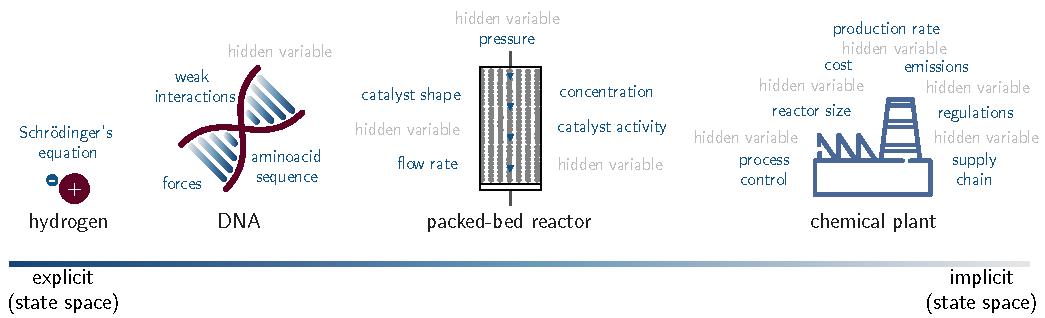
\includegraphics[width=1\textwidth]{figures/rescaled_figures/chemrev_figure1.pdf}   
    \caption{\textbf{State space description for chemistry at different scales}. We illustrate how the number of hidden variables (gray) is growing with scale and complexity. For simple systems we can explicitly write down all variables and their values and perfectly describe the system. For more complex systems---closer to practical applications---we can no longer do that. Many more variables cannot be explicitly enumerated.}
    \label{fig:shape_of_data}
\end{figure}

For phenomena characterized by irreducible complexity, success is often serendipitous. 
As pointed out by \textcite{rulev2017serendipity}, chemical literature commonly contains terms such as \enquote{to our surprise}, \enquote{remarkable reactivity}, or \enquote{unusual performance}, which may reflect the complexity of scientific questions and the diminishing explainability of observed results.

\paragraph{Emergent complexity} In contrast to irreducible complexity, there is a subset of chemical problems for which all relevant parameters can explicitly be listed, but the complexity emerges from the intricate, potentially chaotic, interactions among them. A well-known example is the Belousov-Zhabotinsky reaction, \autocite{Cassani2021BZ} which exhibits oscillations and pattern formation as a result of a complex chemical reaction network. 
Individual chemical reactions within the network are simple, but their interactions create a dynamic, self-organizing system with properties not seen in the individual components.
An example of how fast the parameter space can grow was provided by \textcite{NEURIPS2024_53704142}, who show that a single reaction type and a few hundred molecular building blocks can create tens of thousands of possible solutions. 
When scaling up to only five reaction types, the exploration of the entire space can become intractable, estimated at approximately $10^{22}$ solutions. 
When optimization objectives are involved---finding the shortest synthesis pathway or maximizing the yield---such problems are often NP-hard, meaning that no known polynomial-time algorithms can guarantee optimal solutions, though various heuristic and approximation methods can provide good solutions.

Knowing the ratio between explicit and implicit parameters helps in selecting the appropriate model architecture. 
If most of the variance is caused by explicit factors, these can be incorporated as priors or constraints in the model, thereby increasing data efficiency. 
This strategy can, for instance, be applied in the development of force fields where we know the governing equations and their symmetries, and can use them to enforce such symmetries in the model architecture (as hard restrictions to a family of solutions). \autocite{unke2021machine,Musil_2021}
However, when the variance is dominated by implicit factors, such constraints can no longer be formulated, as the governing relationships are not known. 
In those cases, flexible \glspl{gpm} with soft inductive biases---which guide the model toward preferred solutions without enforcing strict constraints on the solution space\autocite{wilson2025deep}---are more suitable. \glspl{llm} fall into this category.


\subsection{Scale of Chemical Data}
Chemistry is an empirical science in which every prediction bears the burden of proof through experimental validation.\autocite{zunger2019beware} 
However, there is often a mismatch between the realities of a chemistry lab and the datasets on which \gls{ml} models for chemistry are trained. 
Much of current data-driven modeling in chemistry focuses on a few large, structured, and highly-curated datasets where most of the variance is explicit (reducible complexity). 
Such datasets, \modelname{QM9} for example,\autocite{ramakrishnan2014quantum} often come from quantum-chemical computations.
Experimental chemistry, however, tends to have a significantly higher variance and a greater degree of irreducible complexity. 
In addition, since data generation is often expensive, datasets are small, and because science is about doing new things for the first time, many datasets also contain at least some unique variables.

Considering the largest chemistry text dataset, \modelname{ChemPile},\autocite{mirza2025chempile0} we can look at how the largest subsets fare in comparison to the smallest ones (see \Cref{tab:small_large_datasets}). 
The largest dataset is approximately three million times larger than the smallest one.

\begin{table}[!h]
    \centering
    \caption{\textbf{Token counts for the three largest and smallest datasets in the \modelname{ChemPile}\autocite{mirza2025chempile0} collection.} Dominating datasets contribute a large portion of the total token count (a token represents the smallest unit of text that a \gls{ml} model can process), with the small datasets significantly increasing the diversity.}
    \label{tab:dataset-sizes}
    \begin{tabular}{lr}
        \toprule
        \textbf{Dataset} & \textbf{Token count} \\
        \midrule
        \multicolumn{2}{l}{\textit{Three largest ChemPile datasets}} \\
        \midrule
        NOMAD crystal structures\autocite{scheidgen2023nomad} & 5,808,052,794 \\
        \gls{ord}\autocite{Kearnes_2021} reaction prediction & 5,347,195,320 \\
        \modelname{RDKit} molecular features & 5,000,435,822 \\
        \midrule
        \multicolumn{2}{l}{\textit{Three smallest ChemPile datasets}} \\
        \midrule
        Hydrogen storage materials\autocite{hymarcReversibleHydrides} & 1,935 \\
        List of amino-acids\autocite{alberts2002molecular} & 6,000 \\
        \gls{ord}\autocite{Kearnes_2021} recipe yield prediction& 8,372 \\
        \bottomrule
    \end{tabular}
    \label{tab:small_large_datasets}
\end{table}

The prevalence of many small, specialized datasets over large ones is commonly referred to as \enquote{the long tail problem}.\autocite{heidorn2008shedding} 


\begin{figure}[ht]
    \centering
    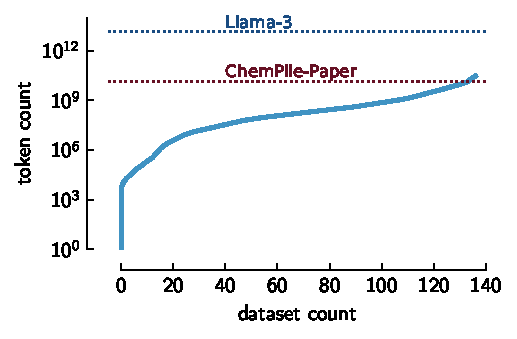
\includegraphics{figures/final_figures/2_DATA_cumulative_histogram.pdf}
    \caption{\textbf{Cumulative token count based on the \modelname{ChemPile} tabular datasets \autocite{mirza2025chempile0}}. We compare the approximate token count for three datasets: \modelname{Llama-3} training dataset,\autocite{grattafiori2024llama} openly available chemistry papers in the \modelname{ChemPile-Paper} dataset, and the \modelname{ChemPile-LIFT} dataset. As can be seen, by aggregating the collection of tabular datasets converted to text format in the \modelname{ChemPile-LIFT} subset, we can achieve the same order of magnitude as the collection of open chemistry papers. However, without smaller datasets, we cannot capture the breadth and complexity of chemistry data, which is essential for training \gls{gpm}. The tokenization method for both \modelname{ChemPile} and \modelname{Llama-3} is provided in the respective papers.}
    \label{fig:scale_of_data}
\end{figure}

This can be seen in \Cref{fig:scale_of_data}. We show that while a few datasets are large, the majority of the corpus consists of small but collectively significant and chemically diverse datasets.
The actual tail of chemical data is even larger, as \Cref{fig:scale_of_data} only shows the distribution for manually curated tabular datasets and not all data actually created in the chemical sciences.
Given that every dataset in the long tail relies on unique sources of variance---it is very difficult to leverage this long tail with conventional \gls{ml} techniques. However, the promise of \glspl{gpm} such as \glspl{llm} is that they can very flexibly integrate and jointly model the diversity of small datasets that exist in the chemical sciences.

\subsection{Dataset Creation}

Before a model can be trained or tested, suitable data must first be collected. 
It is important to note that when working with \glspl{gpm}, data can---but should not---be directly ingested in a raw format and requires some form of pre-processing.
Training \glspl{gpm} typically requires a large and diverse dataset, compiled in a form that can be efficiently ingested by the training pipeline.

Strategies for doing so can be broadly categorized into two groups (see  \Cref{fig:data_protocols}).
One can utilize a \enquote{top-down} approach where a large and diverse pool of data---e.g., results from web-crawled resources such as \modelname{CommonCrawl}\autocite{commoncrawl}---is filtered using custom-built procedures (e.g., using regular expressions or classification models). 
This approach is gaining traction in the development of foundation models such as \glspl{llm}.\autocite{penedo2023refinedweb,penedo2024fineweb,guo2025deepseek} Alongside large filtered datasets, various data augmentation techniques have further increased the performance of \glspl{gpm}.\autocite{maini2024rephrasing,pieler2024rephrasing}

Alternatively, one can take a \enquote{bottom-up} approach by specifically creating novel datasets for a given problem---an approach which has been very popular in \gls{ml} for chemistry. 

In practice, a combination of both approaches is often used. In most cases, key techniques include filtering and the generation of synthetic data.

\begin{figure}[ht]
    \centering
    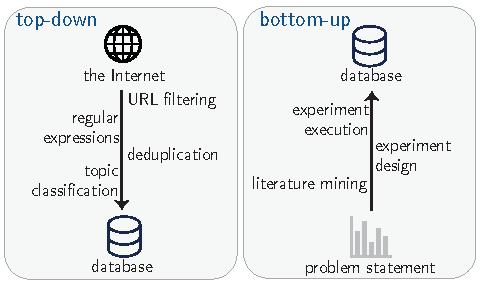
\includegraphics{figures/rescaled_figures/chemrev_figure3.pdf}
    \caption{\textbf{Dataset creation protocols}. In \enquote{top-down} approaches, we curate a large corpus of data, which can be used to train \glspl{gpm}. The \enquote{bottom-up} approach starts from a problem definition, and the dataset can be collected via literature mining and experiments. Both approaches can make use of synthetic data to increase the data size and diversity.}
    \label{fig:data_protocols}
\end{figure}


\subsubsection{Filtering}

\glspl{gpm} are currently trained on very large datasets, enabled by the availability of ever-growing computational resources.\autocite{krizhevsky2012imagenet,kaplan2020scaling, hooker2020hardware, dotan2019value0laden} 
The Internet has been the primary source of dataset construction for \glspl{gpm}. 
While initially the focus was on training on maximally large datasets, empirical evidence has shown that smaller, higher-quality datasets can lead to better results.\autocite{gunasekar2023textbooks, marion2023less} For example, \textcite{shao2024deepseekmath0} filtered \modelname{CommonCrawl} for mathematical text using a combination of regular expressions and a custom, iteratively trained classification model\autocite{bojanowski2017enriching}. 
An alternative approach was pursued by \textcite{thrush2024improving} who introduced a training-free framework. In this method, the pre-training text was chosen by measuring the correlation of each web-domain's perplexity (a metric that measures how well a language model predicts a sequence of text)---as scored by $90$ publicly-available \glspl{llm}---with downstream benchmark accuracy, keeping only the high-correlation domains. 

In the chemical domain, \modelname{ChemPile}\autocite{mirza2025chempile0} is the only open-source, pre-training scale dataset, that underwent several filtering steps. For example, a large subset of the papers in \modelname{ChemPile-Paper} come from the \modelname{Europe PMC} dataset. To filter for chemistry papers, a custom classification model was trained from scratch using topic-labeled data from the \modelname{CAMEL}\autocite{li2023camel} dataset. To evaluate the accuracy of the model ($\text{F1-score}=0.77$), expert-annotated data was used.


\subsubsection{Synthetic Data}
\label{sec:syn-data}

Instead of only relying on existing datasets, one can also leverage techniques for generating synthetic data. 
Generation of synthetic data is often required to augment scarce real-world data, but can also be used to achieve the desired model behavior (e.g., invariance in image-based models).

These approaches can be grouped into rule-based and generative methods. 
Rule-based methods apply manually defined transformations---such as rotations and mirroring---to present different representations of the same instance to a model. 
In contrast, generative augmentation creates new data by applying transformations learned through a \gls{ml} model.

\paragraph{Rule-based augmentation} The transformations applied for generating new data in rule-based approaches vary depending on the modality (e.g., image, text, or audio).  
The most common application of rule-based techniques is on images, via image transformations such as distortion, rotation, blurring, or cropping.\autocite{shorten2019survey} 
In chemistry, tools like \modelname{RanDepict}\autocite{brinkhaus2022randepict} have been used to create enriched datasets of chemical representations. 
These tools generate human-like drawings of chemical structures that mimic the common illustrations found in scientific literature or even in patents (e.g., by applying image templates from different publishers, or emulating the style of older manuscripts) and further augment them using conventional image-augmentation techniques.


Rule-based augmentations can also be applied to text. Early approaches involved simple operations like random word swapping, random synonym replacement, and random deletions or insertions, which are often labeled \enquote{easy augmentation} methods.\autocite{shorten2021text,wei2019eda0}

In chemistry, text templates have been used.\autocite{xie2023darwin,mirza2025chempile0, jablonka2024leveraging, vanherck2025assessment}  
Such templates define a sentence structure with semantically configurable fields, which are then filled using structured tabular data. 
However, it is still unclear how to best construct such templates, as studies have shown that the same data shown in different templates can lead to distinct generalization behavior.\autocite{gonzales2024evaluating} 

We can also apply rule-based augmentation for specific molecular representations (for more details on representations see \Cref{sec:common_representations}). 
For example, the same molecule can be represented with multiple different, yet valid \gls{smiles} strings. 
% The use of all of them can be leveraged to obtain richer latent representations compared to models trained only on canonical \gls{smiles}. 
\textcite{bjerrum2017smiles} used this technique to augment a predictive model, where multiple \gls{smiles} strings were mapped to a single property. 
When averaging the predictions over multiple \gls{smiles} strings, at least a $10\%$ improvement was observed compared to their single \gls{smiles} counterparts. 
Such techniques can be applied to other molecular representations (e.g., \gls{iupac} names or \gls{selfies}), but historically, \gls{smiles} has been used more often. 
As a result, its augmentations have been studied more extensively.\autocite{kimber2021maxsmi,born2023chemical,arus2019randomized}

A broad array of augmentation techniques has been applied to spectral data---from simple noise addition\autocite{ke2018convolutional,moreno2022application} to physics-informed augmentations (e.g., through DFT simulations).\autocite{oviedo2019fast,gao2020general}

\paragraph{Generative augmentation}
In some cases, however, it is not possible to write down the rules. For instance, it is not obvious how text can be transformed into different styles using rules alone.
Recent advances in deep learning have facilitated another, more flexible, approach to synthetic data generation. \autocite{maini2024rephrasing} 
A simple technique is to apply contextual augmentation \autocite{kobayashi2018contextual}, which implies the sampling of synonyms from a probability distribution of a \gls{lm}. 
Another technique is \enquote{back translation},\autocite{edunov2018understanding} a process in which text is translated to another language and then back into the original language to generate semantically similar variants. 
While this technique is typically used within the same language,\autocite{lu2024mathgenie0} it can also be extended to multilingual setups\autocite{hong2024cantonmt0}.
 
Other recent approaches have harnessed auto-formalization\autocite{NEURIPS2022_d0c6bc64}, a \gls{llm}-powered approach that can turn natural-language mathematical proofs into computer-verifiable mathematical languages such as \modelname{Lean}\autocite{de2015lean} or \modelname{Isabelle}\autocite{wenzel2008isabelle}. 
Such datasets have been utilized to advance mathematical capabilities in \glspl{lm}.\autocite{xin2024deepseek,trinh2024solving}

A drawback of generatively augmented data is that its validity is cumbersome to assess at scale, unless it can be verified automatically by a computer program. 
For example, it was demonstrated that an increasing ratio of synthetic data can facilitate model collapse.\autocite{kazdan2024collapse,shumailov2024ai}

Having reviewed the data sources and generation methods, we will, in the following, discuss architectures and training approaches for \glspl{gpm}.